\documentclass[11pt]{article}
\usepackage[textwidth=18.0cm, textheight=23.0cm, top=2.0cm]{geometry}
\usepackage{pst-all}
\usepackage{amssymb}
\usepackage{tikz}
\usepackage{underscore}\begin{document}
\pagestyle{empty}


ClassName: \underline{\textbf{Class_10.2bp-29}}
\par
BinSize: \underline{\textbf{100 × 100}}
\par
ReduceSize: \underline{\textbf{100 × 100}}
\par
TypeNum: \underline{\textbf{59}}
\par
Num: \underline{\textbf{60}}
\par
OutS: \underline{\textbf{80000}}
\par
InS: \underline{\textbf{73074}}
\par
Rate: \underline{\textbf{0.913}}
\par
UB: \underline{\textbf{8}}
\par
LB0: \underline{\textbf{8}}
\par
LB: \underline{\textbf{8}}
\par
LBWithCut: \underline{\textbf{8}}
\par
NodeCut: \underline{\textbf{0}}
\par
ExtendedNodeCnt: \underline{\textbf{1}}
\par
GenNodeCnt: \underline{\textbf{1}}
\par
PrimalNode: \underline{\textbf{0}}
\par
ColumnCount: \underline{\textbf{8}}
\par
TotalCutCount: \underline{\textbf{0}}
\par
RootCutCount: \underline{\textbf{0}}
\par
LPSolverCnt: \underline{\textbf{1}}
\par
PricingSolverCnt: \underline{\textbf{0}}
\par
BranchAndBoundNum: \underline{\textbf{1}}
\par
isOpt: \underline{\textbf{true}}
\par
TimeOnInitSolution: \underline{\textbf{0.190 s}}
\par
TimeOnPrimal: \underline{\textbf{0.000 s}}
\par
TimeOnPricing: \underline{\textbf{0.000 s}}
\par
TimeOnRmp: \underline{\textbf{0.063 s}}
\par
TotalTime: \underline{\textbf{0.330 s}}
\par
\newpage


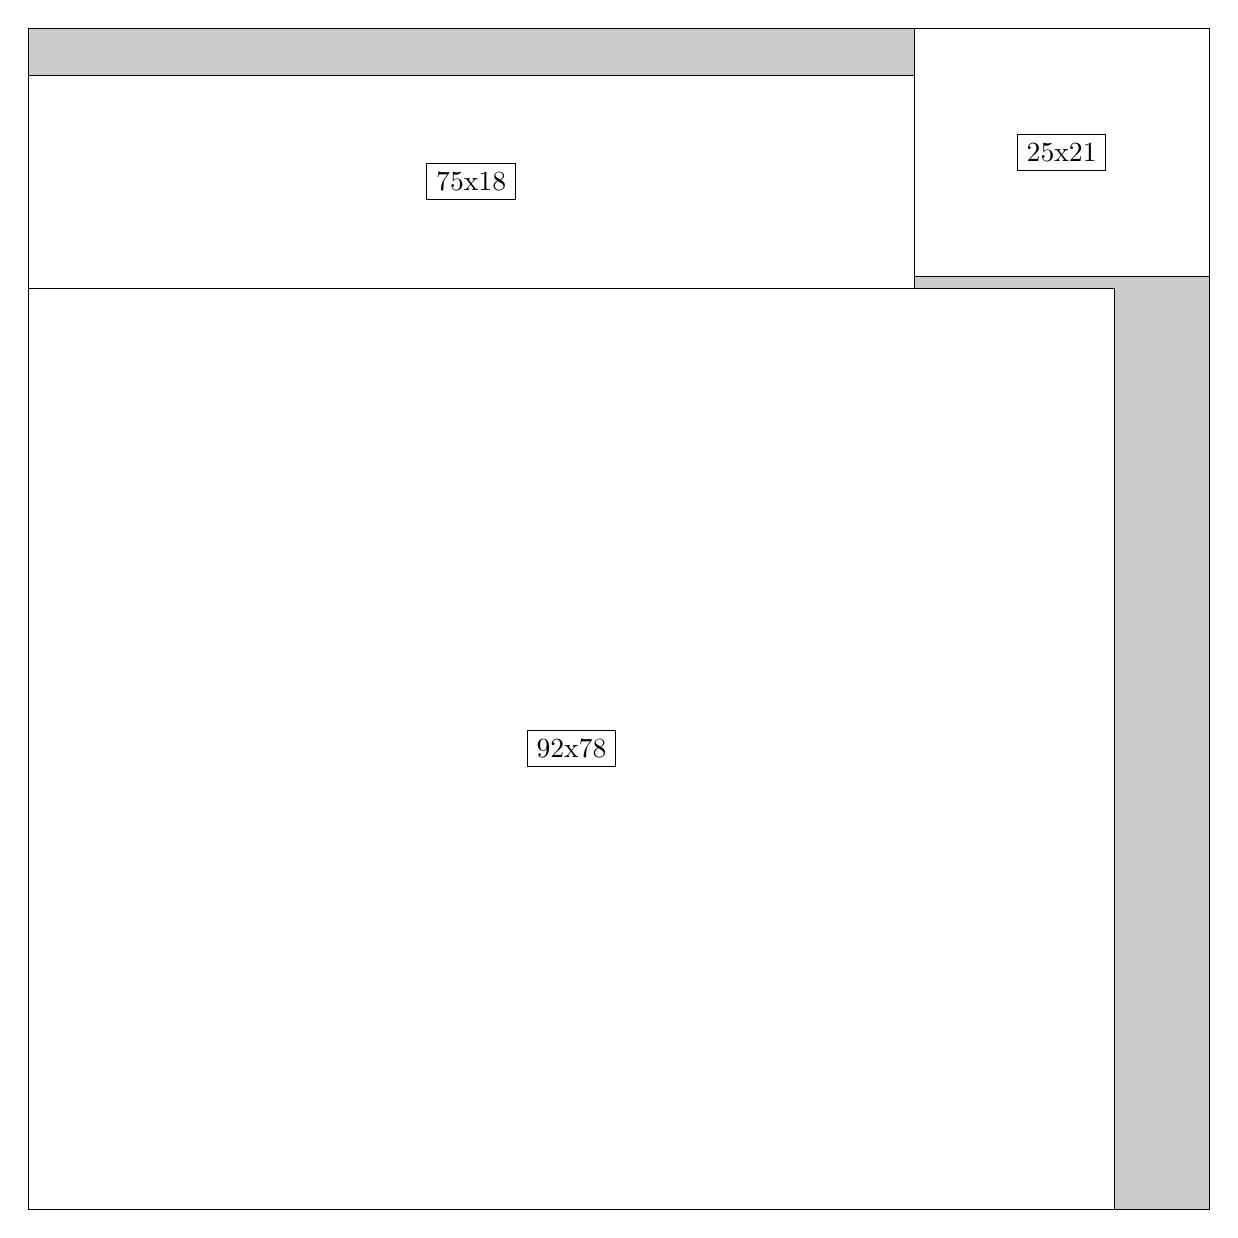
\begin{tikzpicture}[shorten >=1pt,scale=1.0,every node/.style={scale=1.0},->]
\tikzstyle{vertex}=[circle,fill=black!25,minimum size=14pt,inner sep=0pt]
\filldraw[fill=gray!40!white, draw=black] (0,0) rectangle (15.0,15.0);
\foreach \name/\x/\y/\w/\h in {92x78/0.0/0.0/13.799999999999999/11.7,75x18/0.0/11.7/11.25/2.6999999999999997,25x21/11.25/11.85/3.75/3.15}
\filldraw[fill=white!40!white, draw=black] (\x,\y) rectangle node[draw] (\name) {\name} ++(\w,\h);
\end{tikzpicture}


w =92 , h =78 , x =0 , y =0 , v =7176
\par
w =75 , h =18 , x =0 , y =78 , v =1350
\par
w =25 , h =21 , x =75 , y =79 , v =525
\par
\newpage


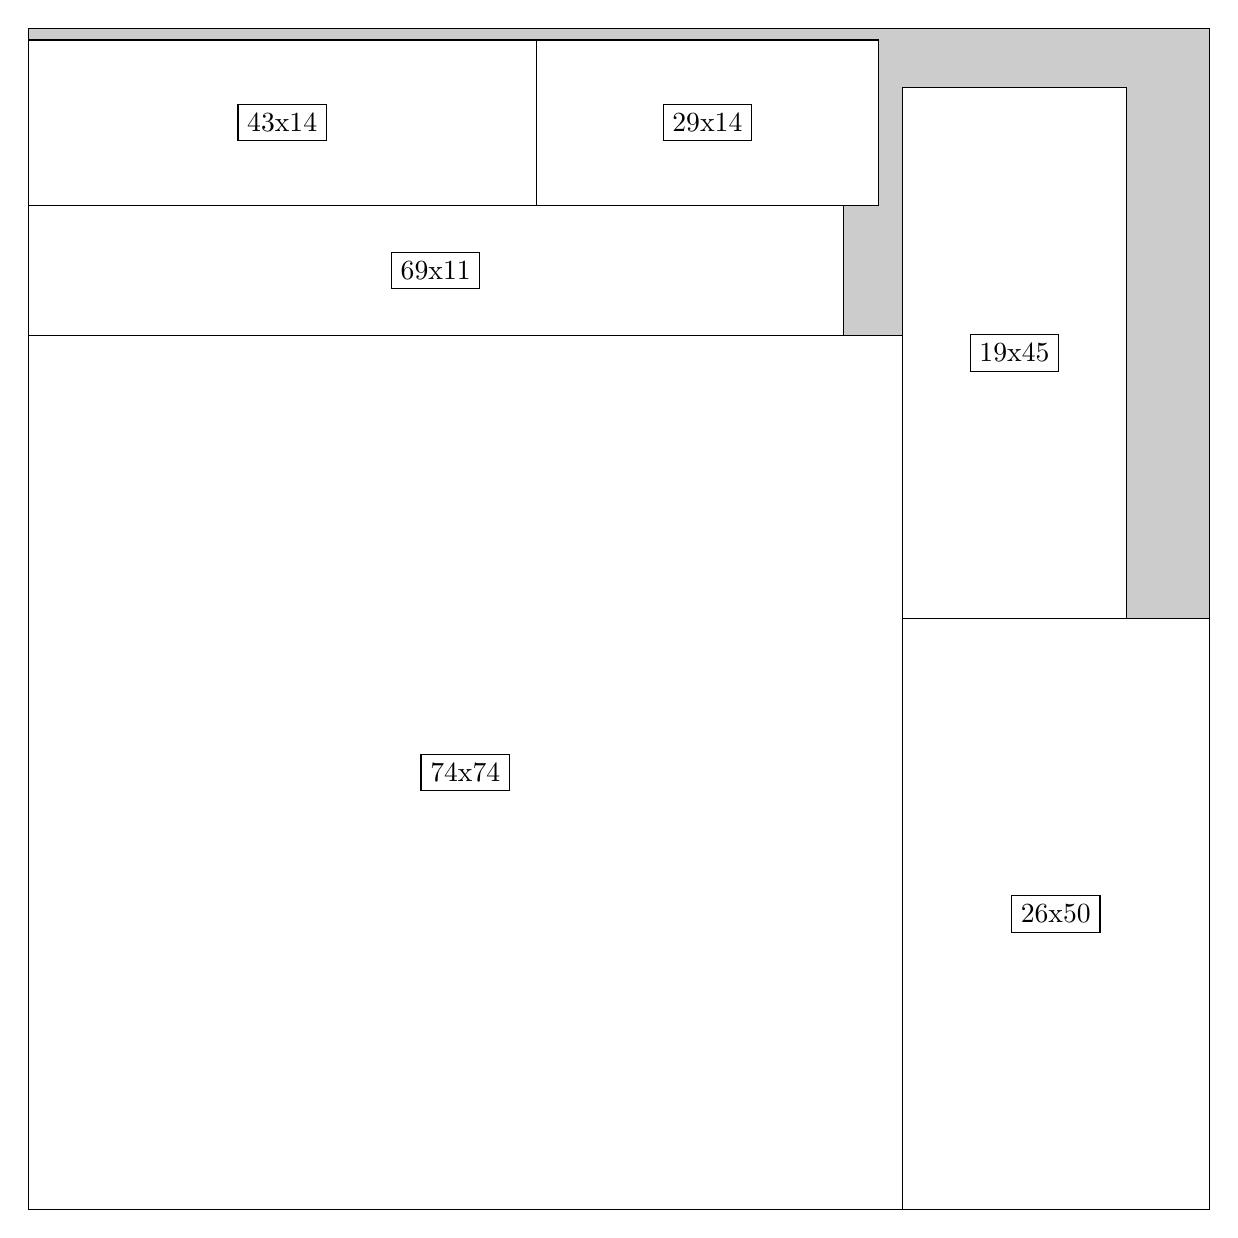
\begin{tikzpicture}[shorten >=1pt,scale=1.0,every node/.style={scale=1.0},->]
\tikzstyle{vertex}=[circle,fill=black!25,minimum size=14pt,inner sep=0pt]
\filldraw[fill=gray!40!white, draw=black] (0,0) rectangle (15.0,15.0);
\foreach \name/\x/\y/\w/\h in {74x74/0.0/0.0/11.1/11.1,26x50/11.1/0.0/3.9/7.5,19x45/11.1/7.5/2.85/6.75,69x11/0.0/11.1/10.35/1.65,43x14/0.0/12.75/6.45/2.1,29x14/6.45/12.75/4.35/2.1}
\filldraw[fill=white!40!white, draw=black] (\x,\y) rectangle node[draw] (\name) {\name} ++(\w,\h);
\end{tikzpicture}


w =74 , h =74 , x =0 , y =0 , v =5476
\par
w =26 , h =50 , x =74 , y =0 , v =1300
\par
w =19 , h =45 , x =74 , y =50 , v =855
\par
w =69 , h =11 , x =0 , y =74 , v =759
\par
w =43 , h =14 , x =0 , y =85 , v =602
\par
w =29 , h =14 , x =43 , y =85 , v =406
\par
\newpage


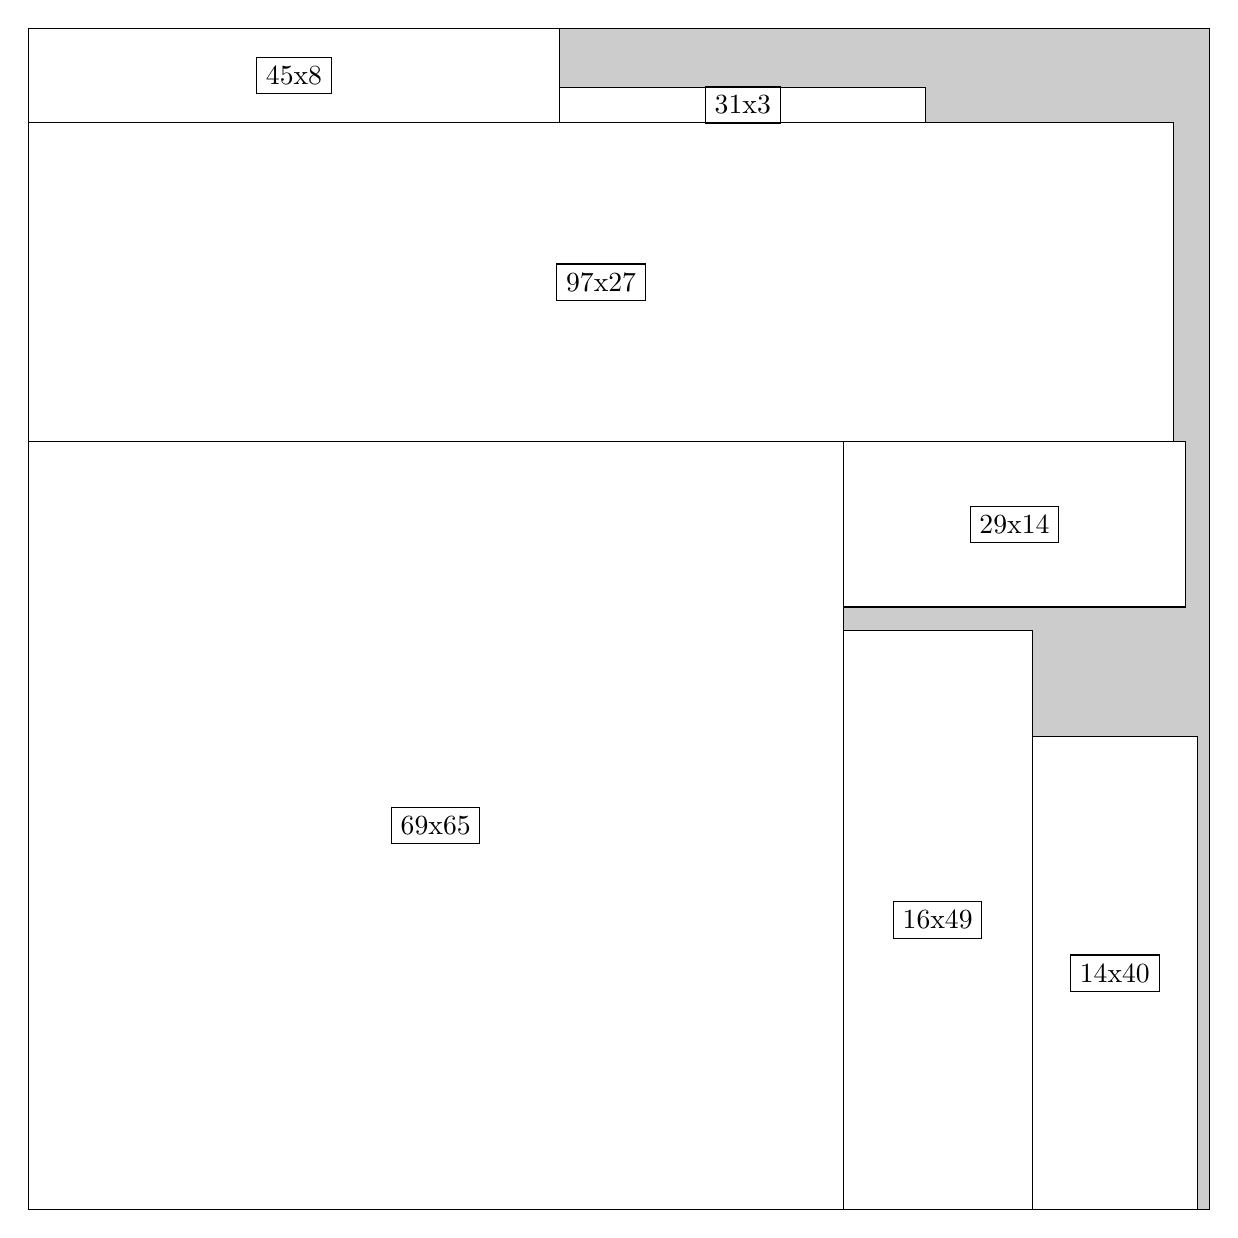
\begin{tikzpicture}[shorten >=1pt,scale=1.0,every node/.style={scale=1.0},->]
\tikzstyle{vertex}=[circle,fill=black!25,minimum size=14pt,inner sep=0pt]
\filldraw[fill=gray!40!white, draw=black] (0,0) rectangle (15.0,15.0);
\foreach \name/\x/\y/\w/\h in {69x65/0.0/0.0/10.35/9.75,97x27/0.0/9.75/14.549999999999999/4.05,16x49/10.35/0.0/2.4/7.35,45x8/0.0/13.799999999999999/6.75/1.2,29x14/10.35/7.6499999999999995/4.35/2.1,14x40/12.75/0.0/2.1/6.0,31x3/6.75/13.799999999999999/4.6499999999999995/0.44999999999999996}
\filldraw[fill=white!40!white, draw=black] (\x,\y) rectangle node[draw] (\name) {\name} ++(\w,\h);
\end{tikzpicture}


w =69 , h =65 , x =0 , y =0 , v =4485
\par
w =97 , h =27 , x =0 , y =65 , v =2619
\par
w =16 , h =49 , x =69 , y =0 , v =784
\par
w =45 , h =8 , x =0 , y =92 , v =360
\par
w =29 , h =14 , x =69 , y =51 , v =406
\par
w =14 , h =40 , x =85 , y =0 , v =560
\par
w =31 , h =3 , x =45 , y =92 , v =93
\par
\newpage


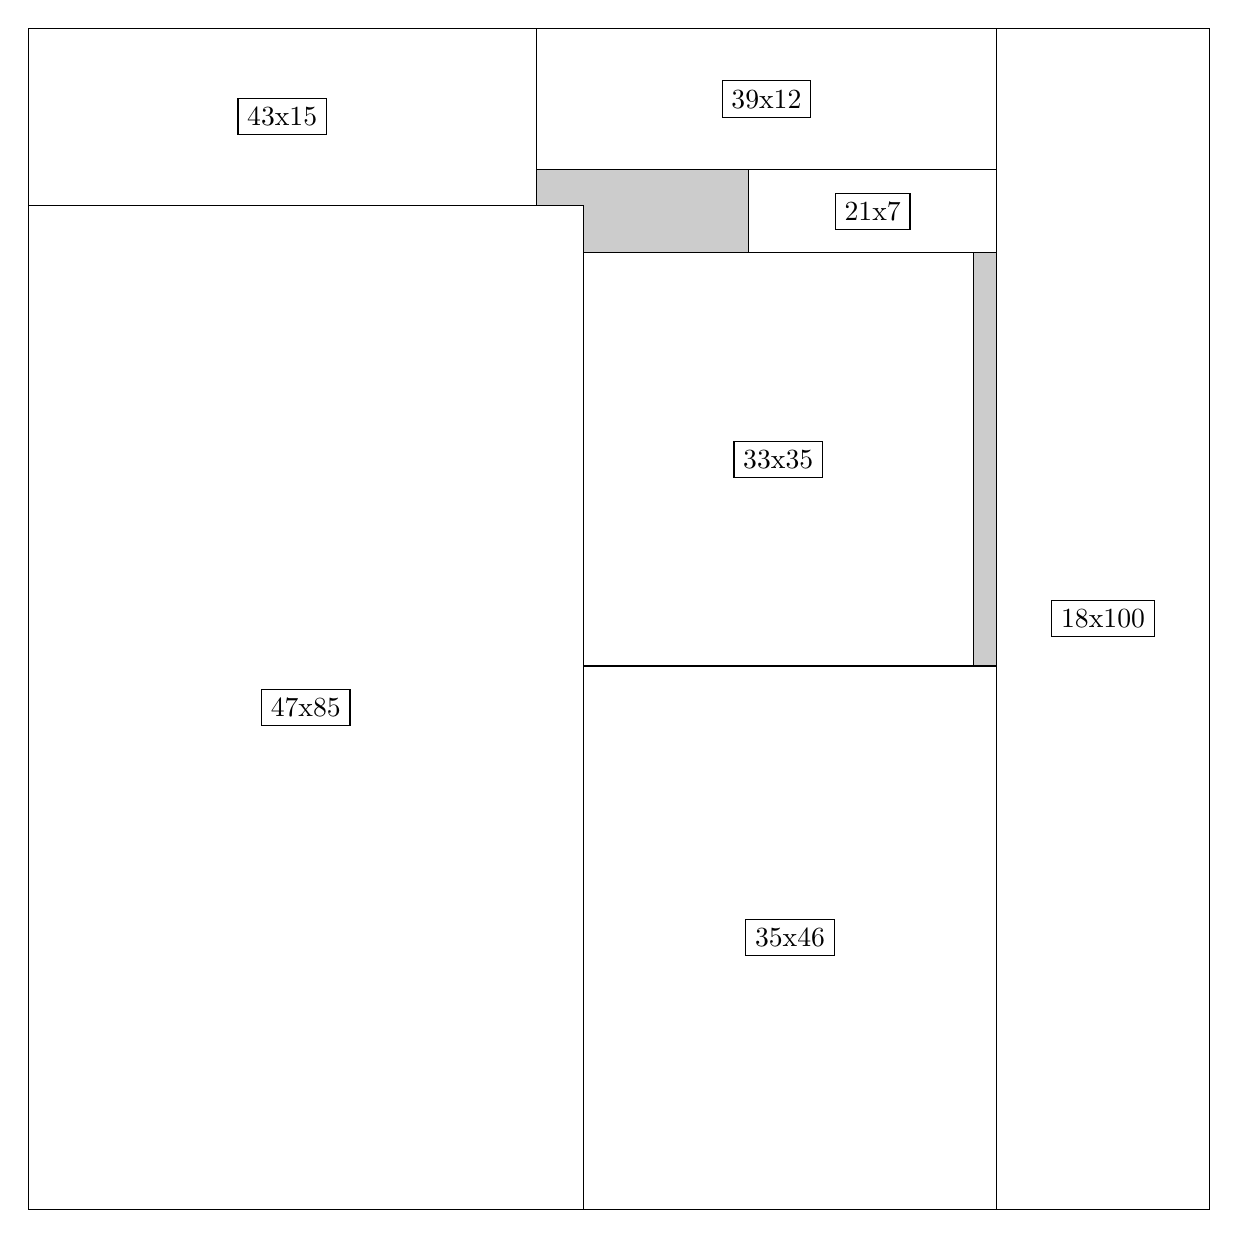
\begin{tikzpicture}[shorten >=1pt,scale=1.0,every node/.style={scale=1.0},->]
\tikzstyle{vertex}=[circle,fill=black!25,minimum size=14pt,inner sep=0pt]
\filldraw[fill=gray!40!white, draw=black] (0,0) rectangle (15.0,15.0);
\foreach \name/\x/\y/\w/\h in {47x85/0.0/0.0/7.05/12.75,18x100/12.299999999999999/0.0/2.6999999999999997/15.0,35x46/7.05/0.0/5.25/6.8999999999999995,33x35/7.05/6.8999999999999995/4.95/5.25,43x15/0.0/12.75/6.45/2.25,39x12/6.45/13.2/5.85/1.7999999999999998,21x7/9.15/12.15/3.15/1.05}
\filldraw[fill=white!40!white, draw=black] (\x,\y) rectangle node[draw] (\name) {\name} ++(\w,\h);
\end{tikzpicture}


w =47 , h =85 , x =0 , y =0 , v =3995
\par
w =18 , h =100 , x =82 , y =0 , v =1800
\par
w =35 , h =46 , x =47 , y =0 , v =1610
\par
w =33 , h =35 , x =47 , y =46 , v =1155
\par
w =43 , h =15 , x =0 , y =85 , v =645
\par
w =39 , h =12 , x =43 , y =88 , v =468
\par
w =21 , h =7 , x =61 , y =81 , v =147
\par
\newpage


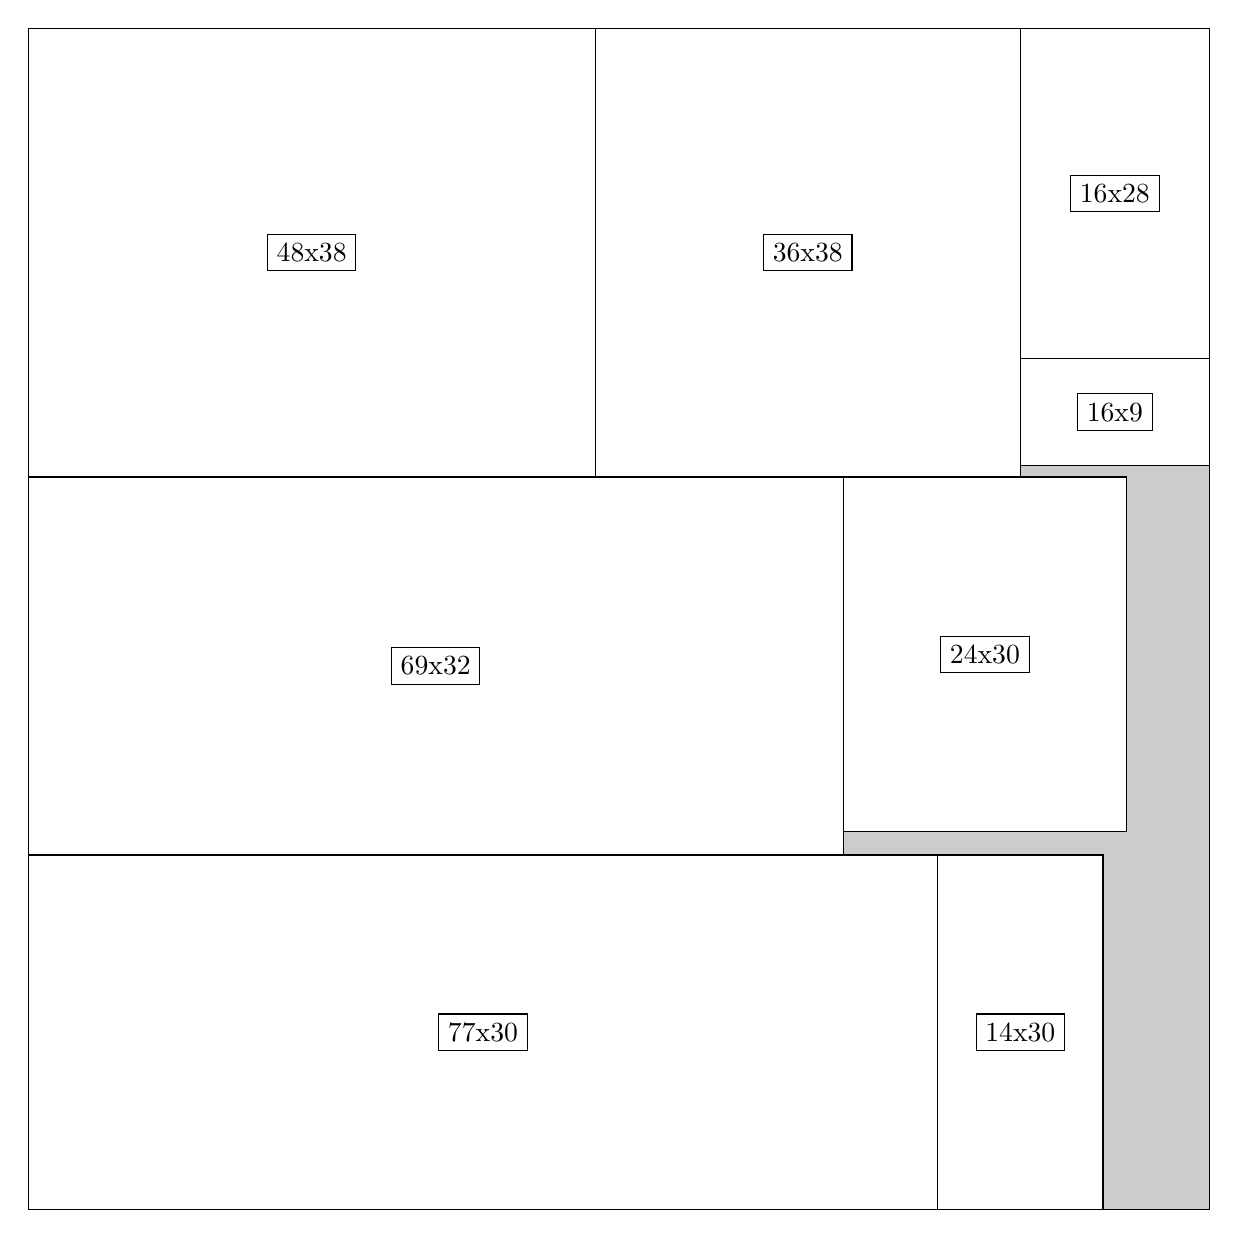
\begin{tikzpicture}[shorten >=1pt,scale=1.0,every node/.style={scale=1.0},->]
\tikzstyle{vertex}=[circle,fill=black!25,minimum size=14pt,inner sep=0pt]
\filldraw[fill=gray!40!white, draw=black] (0,0) rectangle (15.0,15.0);
\foreach \name/\x/\y/\w/\h in {77x30/0.0/0.0/11.549999999999999/4.5,69x32/0.0/4.5/10.35/4.8,48x38/0.0/9.299999999999999/7.199999999999999/5.7,36x38/7.199999999999999/9.299999999999999/5.3999999999999995/5.7,24x30/10.35/4.8/3.5999999999999996/4.5,16x28/12.6/10.799999999999999/2.4/4.2,14x30/11.549999999999999/0.0/2.1/4.5,16x9/12.6/9.45/2.4/1.3499999999999999}
\filldraw[fill=white!40!white, draw=black] (\x,\y) rectangle node[draw] (\name) {\name} ++(\w,\h);
\end{tikzpicture}


w =77 , h =30 , x =0 , y =0 , v =2310
\par
w =69 , h =32 , x =0 , y =30 , v =2208
\par
w =48 , h =38 , x =0 , y =62 , v =1824
\par
w =36 , h =38 , x =48 , y =62 , v =1368
\par
w =24 , h =30 , x =69 , y =32 , v =720
\par
w =16 , h =28 , x =84 , y =72 , v =448
\par
w =14 , h =30 , x =77 , y =0 , v =420
\par
w =16 , h =9 , x =84 , y =63 , v =144
\par
\newpage


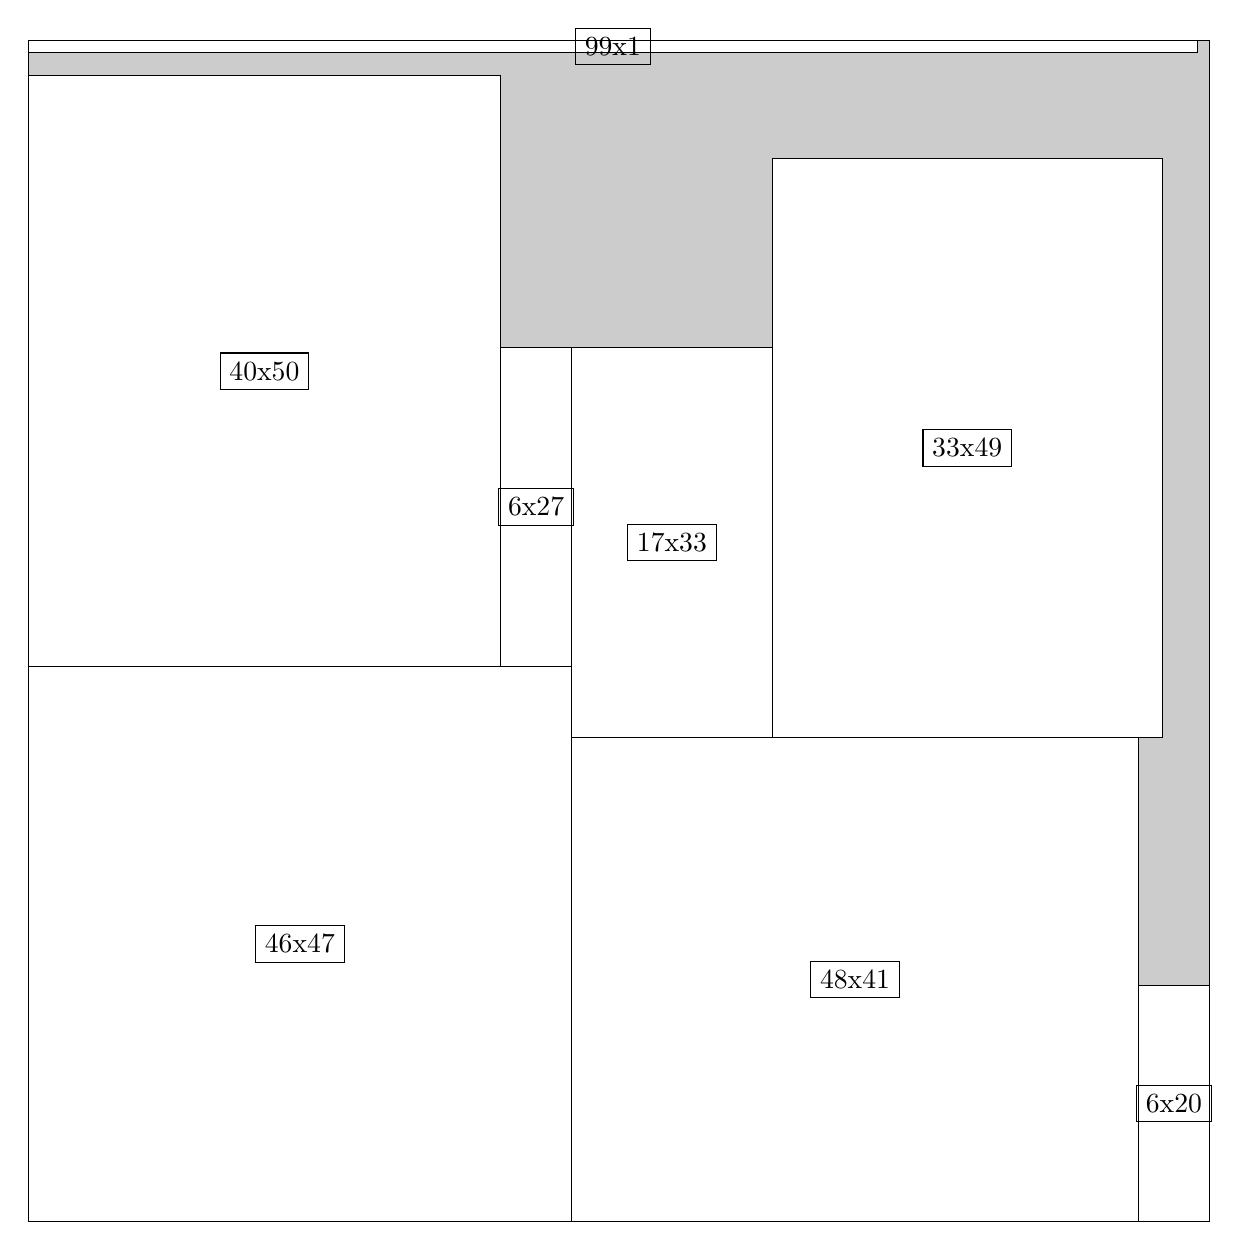
\begin{tikzpicture}[shorten >=1pt,scale=1.0,every node/.style={scale=1.0},->]
\tikzstyle{vertex}=[circle,fill=black!25,minimum size=14pt,inner sep=0pt]
\filldraw[fill=gray!40!white, draw=black] (0,0) rectangle (15.0,15.0);
\foreach \name/\x/\y/\w/\h in {46x47/0.0/0.0/6.8999999999999995/7.05,40x50/0.0/7.05/6.0/7.5,48x41/6.8999999999999995/0.0/7.199999999999999/6.1499999999999995,33x49/9.45/6.1499999999999995/4.95/7.35,17x33/6.8999999999999995/6.1499999999999995/2.55/4.95,6x27/6.0/7.05/0.8999999999999999/4.05,6x20/14.1/0.0/0.8999999999999999/3.0,99x1/0.0/14.85/14.85/0.15}
\filldraw[fill=white!40!white, draw=black] (\x,\y) rectangle node[draw] (\name) {\name} ++(\w,\h);
\end{tikzpicture}


w =46 , h =47 , x =0 , y =0 , v =2162
\par
w =40 , h =50 , x =0 , y =47 , v =2000
\par
w =48 , h =41 , x =46 , y =0 , v =1968
\par
w =33 , h =49 , x =63 , y =41 , v =1617
\par
w =17 , h =33 , x =46 , y =41 , v =561
\par
w =6 , h =27 , x =40 , y =47 , v =162
\par
w =6 , h =20 , x =94 , y =0 , v =120
\par
w =99 , h =1 , x =0 , y =99 , v =99
\par
\newpage


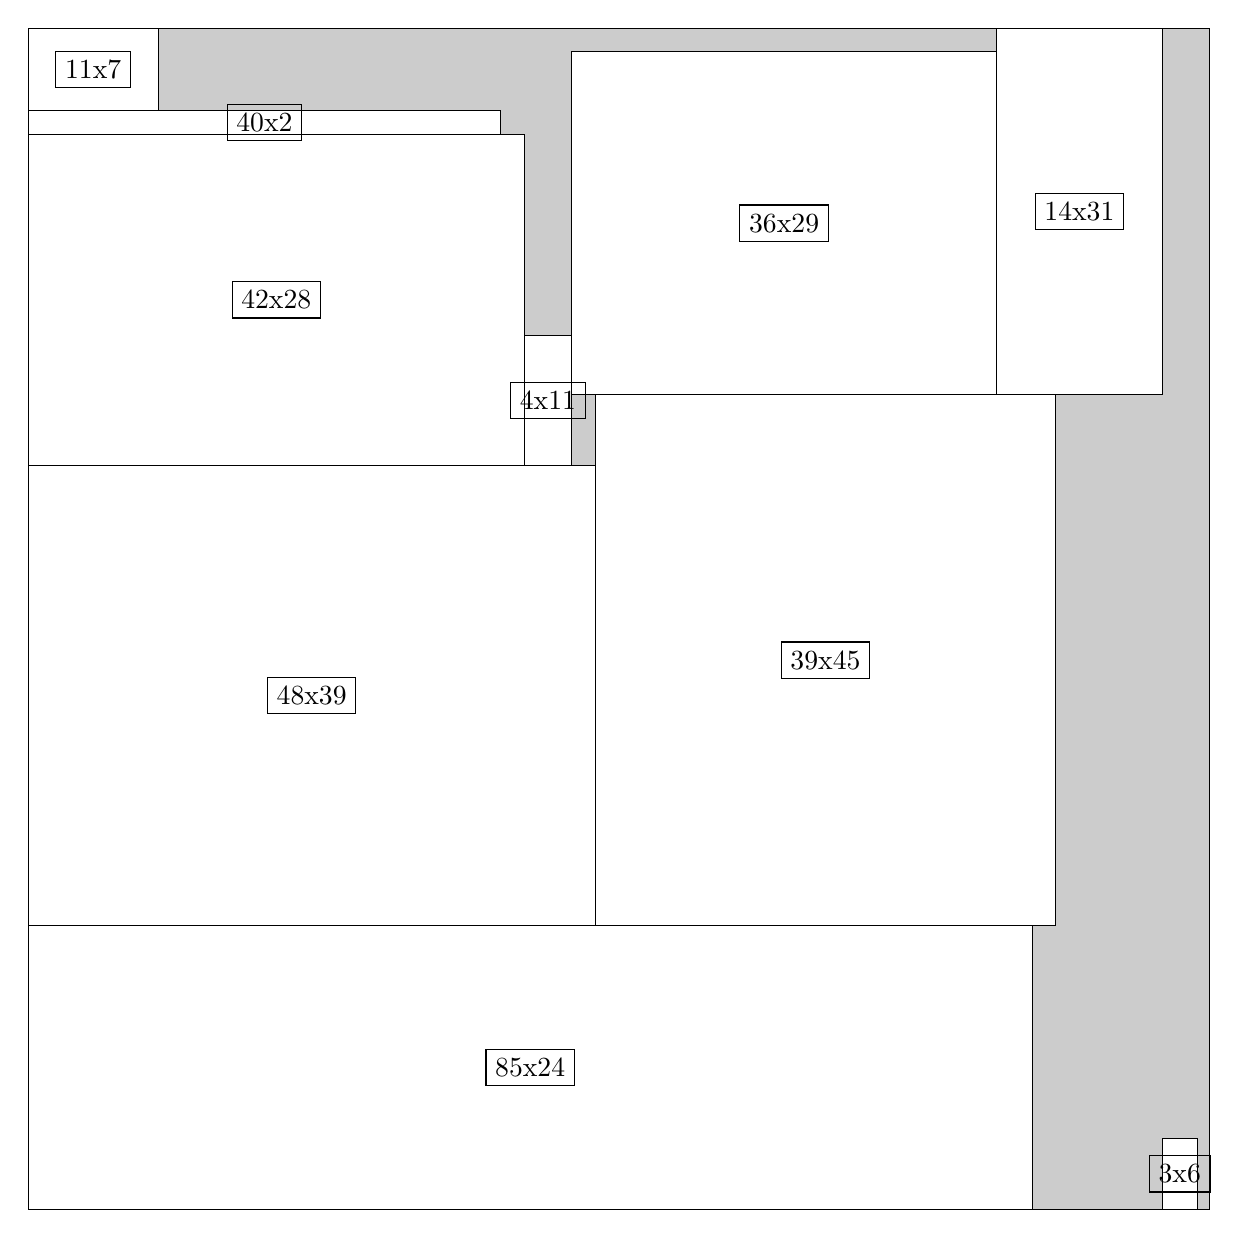
\begin{tikzpicture}[shorten >=1pt,scale=1.0,every node/.style={scale=1.0},->]
\tikzstyle{vertex}=[circle,fill=black!25,minimum size=14pt,inner sep=0pt]
\filldraw[fill=gray!40!white, draw=black] (0,0) rectangle (15.0,15.0);
\foreach \name/\x/\y/\w/\h in {85x24/0.0/0.0/12.75/3.5999999999999996,48x39/0.0/3.5999999999999996/7.199999999999999/5.85,39x45/7.199999999999999/3.5999999999999996/5.85/6.75,42x28/0.0/9.45/6.3/4.2,36x29/6.8999999999999995/10.35/5.3999999999999995/4.35,14x31/12.299999999999999/10.35/2.1/4.6499999999999995,40x2/0.0/13.65/6.0/0.3,11x7/0.0/13.95/1.65/1.05,4x11/6.3/9.45/0.6/1.65,3x6/14.399999999999999/0.0/0.44999999999999996/0.8999999999999999}
\filldraw[fill=white!40!white, draw=black] (\x,\y) rectangle node[draw] (\name) {\name} ++(\w,\h);
\end{tikzpicture}


w =85 , h =24 , x =0 , y =0 , v =2040
\par
w =48 , h =39 , x =0 , y =24 , v =1872
\par
w =39 , h =45 , x =48 , y =24 , v =1755
\par
w =42 , h =28 , x =0 , y =63 , v =1176
\par
w =36 , h =29 , x =46 , y =69 , v =1044
\par
w =14 , h =31 , x =82 , y =69 , v =434
\par
w =40 , h =2 , x =0 , y =91 , v =80
\par
w =11 , h =7 , x =0 , y =93 , v =77
\par
w =4 , h =11 , x =42 , y =63 , v =44
\par
w =3 , h =6 , x =96 , y =0 , v =18
\par
\newpage


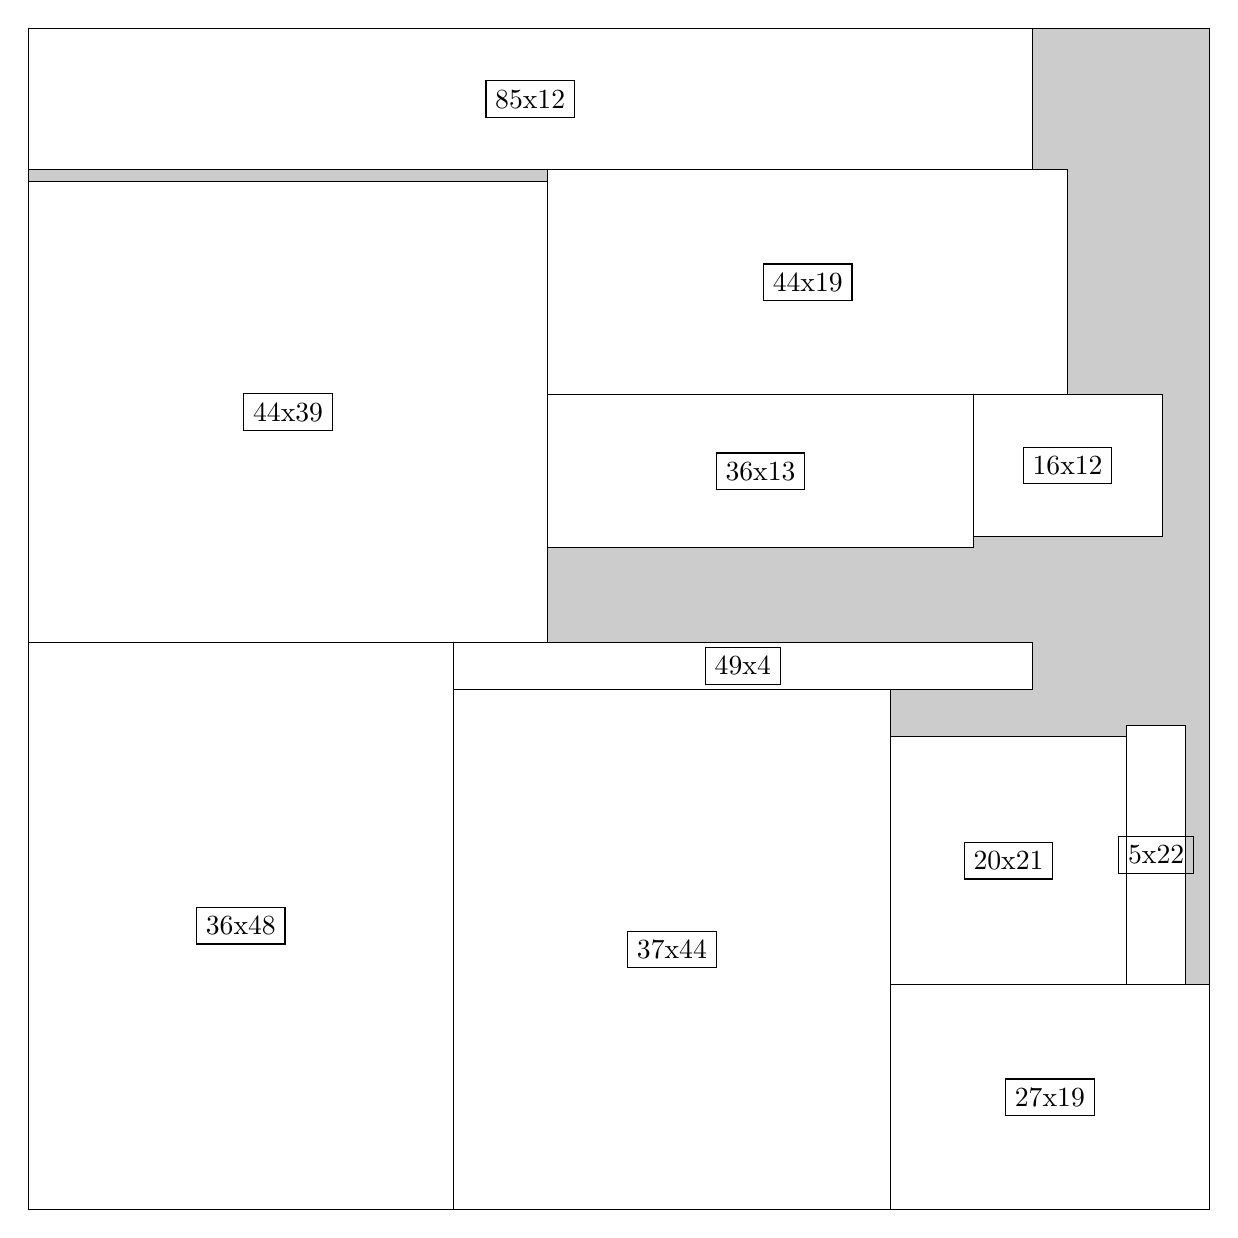
\begin{tikzpicture}[shorten >=1pt,scale=1.0,every node/.style={scale=1.0},->]
\tikzstyle{vertex}=[circle,fill=black!25,minimum size=14pt,inner sep=0pt]
\filldraw[fill=gray!40!white, draw=black] (0,0) rectangle (15.0,15.0);
\foreach \name/\x/\y/\w/\h in {36x48/0.0/0.0/5.3999999999999995/7.199999999999999,44x39/0.0/7.199999999999999/6.6/5.85,37x44/5.3999999999999995/0.0/5.55/6.6,85x12/0.0/13.2/12.75/1.7999999999999998,44x19/6.6/10.35/6.6/2.85,27x19/10.95/0.0/4.05/2.85,36x13/6.6/8.4/5.3999999999999995/1.95,20x21/10.95/2.85/3.0/3.15,49x4/5.3999999999999995/6.6/7.35/0.6,16x12/12.0/8.549999999999999/2.4/1.7999999999999998,5x22/13.95/2.85/0.75/3.3}
\filldraw[fill=white!40!white, draw=black] (\x,\y) rectangle node[draw] (\name) {\name} ++(\w,\h);
\end{tikzpicture}


w =36 , h =48 , x =0 , y =0 , v =1728
\par
w =44 , h =39 , x =0 , y =48 , v =1716
\par
w =37 , h =44 , x =36 , y =0 , v =1628
\par
w =85 , h =12 , x =0 , y =88 , v =1020
\par
w =44 , h =19 , x =44 , y =69 , v =836
\par
w =27 , h =19 , x =73 , y =0 , v =513
\par
w =36 , h =13 , x =44 , y =56 , v =468
\par
w =20 , h =21 , x =73 , y =19 , v =420
\par
w =49 , h =4 , x =36 , y =44 , v =196
\par
w =16 , h =12 , x =80 , y =57 , v =192
\par
w =5 , h =22 , x =93 , y =19 , v =110
\par
\newpage


\end{document}